\documentclass{article}

\usepackage{amsmath}
\usepackage{amssymb}
\usepackage{amsfonts}
\usepackage{mathtools}

\usepackage[thmmarks, amsmath]{ntheorem}

\usepackage{graphicx}
\usepackage{float}

\usepackage{diffcoeff}
\diffdef{}{op-symbol=\mathrm{d},op-order-sep=0mu}

\usepackage{cancel}
\usepackage{interval}

\usepackage{array}

\usepackage{enumitem}

\setlist[enumerate,1]{label=(\alph*)}

\title{Algebraic Topology Homework 3}
\author{Duarte Maia}
%\date{}

\theoremstyle{plain}
\theorembodyfont{\upshape}
\theoremseparator{.}
\newtheorem{theorem}{Theorem}
\newtheorem{prop}{Prop}
\renewtheorem*{prop*}{Prop}
\newtheorem{lemma}{Lemma}
\newtheorem*{ex}{Exercise}

\theoremstyle{nonumberplain}
\theoremheaderfont{\itshape}
\theorembodyfont{\upshape}
\theoremseparator{:}
\theoremsymbol{\ensuremath{\blacksquare}}
\newtheorem{proof}{Proof}
\newtheorem{sol}{Solution}

\theoremsymbol{\text{\textit{(End proof of lemma)}}}
\newtheorem{lemmaproof}{Proof of lemma}

\newcommand{\R}{\mathbb{R}}
\newcommand{\C}{\mathbb{C}}
\newcommand{\Z}{\mathbb{Z}}
\newcommand{\Q}{\mathbb{Q}}

\newcommand{\RP}{\mathbb{RP}}

\newcommand{\kk}{\Bbbk}

\newcommand{\PP}{\mathbb{P}}
\newcommand{\FF}{\mathcal{F}}

\newcommand{\I}{\mathrm{i}}
\newcommand{\e}{\mathrm{e}}

\newcommand{\id}{\mathrm{id}}

\newcommand{\conj}[1]{\overline{#1}}
\newcommand{\close}[1]{\overline{#1}}

\DeclareMathOperator{\inte}{int}
\DeclareMathOperator{\codim}{codim}
\newcommand{\grad}{\nabla}


\DeclareMathOperator{\spec}{spec}

\DeclarePairedDelimiter{\abs}{\lvert}{\rvert}
\DeclarePairedDelimiter{\norm}{\lvert}{\rvert}
\DeclarePairedDelimiter{\Norm}{\lVert}{\rVert}
\DeclarePairedDelimiter{\braket}{\langle}{\rangle}


\begin{document}
\maketitle

\begin{ex}[2.1:3]
Construct a $\Delta$-complex structure on $\RP^n$.
\end{ex}

\begin{sol}
We begin by building a $\Delta$-complex structure on $S^n$. The vertices are the vectors $\pm e_i$, where $e_i$ is the $i$-th canonical basis vector on $\R^{n+1}$. Now, the $k$-th dimensional simplices in this structure are given by the convex hulls of all possible combinations of $k$ distinct vectors $\pm e_i$, with the restriction that a valid combination may not contain $+ e_i$ and $- e_i$ at the same time. To set orientations, we order the vertices as follows: $-e_1 < +e_1 < -e_2 < +e_2 < \dots$ It is easy to verify that this construction is closed under faces.

Now, we take the quotient by the antipodal map. Note that the antipodal map preserves simplices (obviously) and their orientations (because it preserves the order on admissible sets of vertices), so we are identifying simplices in a way that preserves the $\Delta$-structure, and thus we obtain a legitimate new $\Delta$-complex, which is the structure on $\RP^n$ we sought.
\end{sol}

\begin{ex}[2.1:7]
Find a $\Delta$-structure on $S^3$ with a single $3$-simplex. Compute its simplicial homology.
\end{ex}

\begin{sol}
Let the $3$-simplex be $[0123]$, and identify the faces $[012] \sim [013]$ and $[023] \sim [123]$. We claim that the resulting object is $S^3$.

To prove this claim, we do one identification at a time, say the second one. Then, the result is fortunately embeddable in $\R^3$ and looks like the following picture.
\begin{figure}[H]
\centering
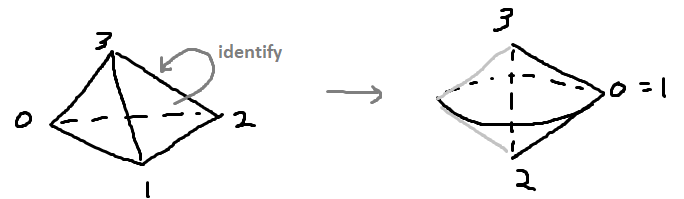
\includegraphics[width=\linewidth]{s31}
\end{figure}

The next identification will simply identify the top face with the bottom face, so it suffices to show the following fact: If we identify the top and bottom hemispheres of $\close {D^3}$ by vertical projection, we obtain $S^3$.

To show this fact, we begin by recalling that $\close{D^3}$ may be seen as $S^2 \times I$ with one of the bases collapsed. We may represent $S^2 \times I$ in $\R^3$ as follows.
\begin{figure}[H]
\centering
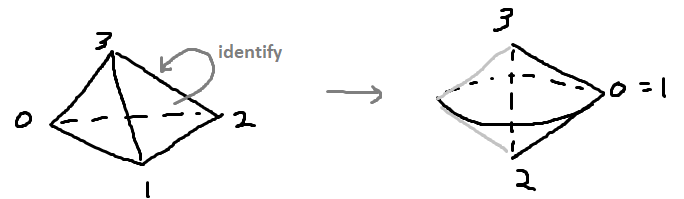
\includegraphics[width=\linewidth]{s31}
\end{figure}

Now, the figure we are interested in consists of collapsing one of the $S^2$ faces of the above figure to a point (to get $\close{D^3}$) and collapsing the other by vertical projection (to get the thing we want to show is $S^3$). However, identifications fortunately commute, so we begin by doing the second identification, and moreover since both bases are equivalent (we can flip the figure inside out) we may perform this identification on the inside $S^2$.

It is easy to see that we obtain a copy of $\close{D^3}$, with the collapsed $S^2$ looking like a $\close{D^2}$ floating inside $\close{D^3}$. Now, we collapse the border of $\close{D^3}$, and it is a known fact that the resulting figure is $S^3$.

\smallskip

Let us now compute the singular homology. Under the identifications of the faces above, we have the identifications of vertices
\begin{equation}
[0] = [1], \quad [2] = [3],
\end{equation}
together with the associated identifications of edges, so that there are three edges in total: $[01]$, $[02] = [03] = [12] = [13]$, and $[23]$. Thus, we may compute the homology groups.
\begin{equation}
\begin{cases}
H_3 = \braket{[0123] \mid [123] - [023] + [013] - [012] = 0} = \braket{[0123]} \cong \Z,\\
H_2 = 0 \quad \text{(The $\partial$ map is injective)}\\
\begin{multlined}
H_1 = \braket{[01], [23] \mid [01] - [02] + [12] = 0, [02] - [03] + [23] = 0}\\[-3.5ex]
= \braket{[01], [23] \mid [01] = 0, [23] = 0} = 0,
\end{multlined}\\
H_0 = \braket{[0], [2] \mid [0] - [0] = 0, [0] - [2] = 0, [2] - [2] = 0} = \braket{[0]} \cong \Z.
\end{cases}
\end{equation}

This completes the solution of the exercise.
\end{sol}

\begin{ex}[2.1:8]
Let $X$ be a $3$-dimensional complex built from $n$ tetrahedra as in Hatcher. Compute the simplicial homology of $X$.
\end{ex}

\begin{sol}{}
[Note: Hatcher is ambiguous about which direction the tetrahedra are ordered. To disambiguate, we adopt the convention that they are numbered according to the right-hand rule, with the thumb facing up.]

First, let us take stock of the simplices at hand. There are $n$ tetrahedra, $T_1$ to $T_n$. Each tetrahedron has four faces, but they suffer heavy identifications. For one, the `side faces' coincide with side faces of neighboring tetrahedra. Thus, there are exactly $n$ `side faces'; we call $S_1, \dots, S_n$ these faces, and $S_i$ is the face that lies between $T_i$ and $T_{i+1}$ (indices mod $n$). Moreover, there are also `top' and `bottom' faces, but by the identifications it suffices only to name the bottom faces. Let $B_i$ be the bottom face of $T_i$.

Now, let us look at the edges. There is one edge in the center going from bottom to top; we call it $c$. Then, for each side face $S_i$, there exist two edges, one below and one on top, but using an argument similar to the top/bottom faces, it suffices to name the bottom edges, call them $b_i$. Finally, there is exactly one outside edge: the top/bottom face identifications ensure that the edge going `around the lens' is just one edge repeated several times. We call it $e$.

Finally, there are only two vertices. The top vertex $1$ (which is identified with the bottom vertex) and the outside vertex $2$.

We now effectively have all the chains of all dimensions, so we need to compute the border operators. Let us start with $\partial \colon C_3 \to C_2$. It is given on the generators by
\begin{equation}\label{eq:eq1}
\partial(T_i) = S_i - S_{i-1} + B_{i-1} - B_i.
\end{equation}

Therefore, we may compute $H_3 = Z_3$ by computing the kernel of this $\partial$ map. In order for $\partial(\text{something})$ to equal zero, we need all terms $S_i$ to cancel out as a cyclic telescopic sum, so the only way for this to happen is for all $T_i$ to contribute equally. Hence,
\begin{equation}
H_3 = \braket{T_1 + \dots + T_N} \cong \Z.
\end{equation}

Now, let us compute $Z_2$, and to do so, we compute $\partial \colon C_2 \to C_1$. It is given by
\begin{equation}\label{eq:eq2}
\begin{aligned}
\partial(S_i) &= c - b_{i-1} + b_i,\\
\partial(B_i) &= b_i - b_{i-1} + e.
\end{aligned}
\end{equation}

Hence, the kernel of this map is described as follows. Let $z = \sum x_i S_i + y_i B_i$ be an element of $C_2$. For it to be in the kernel, the $c$ component of the border must be null, hence $\sum x_i = 0$. Likewise, $\sum y_i = 0$. Finally, the $b_i$ component must be null, so $x_i + y_i = x_{i+1} + y_{i+1}$. Chaining these equalities together, we conclude that $x_i + y_i$ is actually a parameter of $z$, and so it is actually of the form
\begin{equation}
z = \sum x_i S_i + (C - x_i) B_i,
\end{equation}
where $C$ is an integer.

Now, using the condition that $\sum x_i = \sum y_i = 0$, it is easy to conclude that $C = 0$, and so we finally have characterized the kernel: it is given by elements of the form $z = \sum x_i (S_i - B_i)$ with $\sum x_i = 0$. In other words, it is generated by elements of the form $S_i - B_i - S_{i+1} + B_{i+1}$, but by \eqref{eq:eq1} these are all in $B_2$, hence $H_2 = 0$.

Let us now look at $Z_1$. To do so, we compute $\partial \colon C_1 \to C_2$. It is given by
\begin{equation}
\begin{aligned}
\partial(c) &= 0,\\
\partial(b_i) &= 1-2,\\
\partial(e) &= 0.
\end{aligned}
\end{equation}

Thus, the kernel is generated by $c$, $e$, and elements of the form $b_i - b_{i+1}$, but, note, not freely! To let it be freely generated, we exclude $b_n - b_1$ from the list.

Now, note that by \eqref{eq:eq2}, in homology all $b_i - b_{i+1}$ are identified with $c$ and $e$ at the same time, and hence with each other. Therefore, all but one generator is redundant, and we may remove all those other generators and the relations that say that they are all the same. At the end, we still have one relation though, which is given by $c = b_n - b_1$ (well, there is another similar relation for $e$, but in light of equality of the generators they are equivalent). Now, this last relation may be written purely in terms of $c$, using a telescopic sum in the $b_i$, and it will give us that $nc = 0$. Thus, $H_1$ is presented as $\braket{c \mid nc = 0} \cong \Z_n$.

Finally, $H_0 = \braket{1,2} / B_0$, and $B_0$ is generated by $1-2$, so $H_0$ has exactly one generator and is therefore isomorphic to $\Z$.
\end{sol}

\begin{ex}[2.1:12]
Show that chain homotopy is an equivalence relation.
\end{ex}

\begin{sol}
Let $f, g, h \colon C_* \to D_*$ and $F, G \colon C_* \to D_{*+1}$ be chain homotopies between $f$ and $g$, and $g$ and $h$ respectively. We show that $f$ and $h$ are homotopic by building a chain homotopy between them, namely $F+G$. Indeed, it is trivial to verify this:
\begin{equation}
\begin{aligned}
\partial(F+G) + (F+G)\partial &= \partial F + F \partial + \partial G + G \partial \\
&= g - f + h - g \\
&= h - f.
\end{aligned}
\end{equation}

Proof complete.
\end{sol}

\begin{ex}[2.1:15]
Show that if $A \to B \to C \to D \to E$ is exact, $C = 0$ iff $A \to B$ is surjective and $D \to E$ is injective. Conclude that an inclusion $A \hookrightarrow X$ induces a homomorphism in homology iff the relative homology is null.
\end{ex}

\begin{sol}
($\rightarrow$) Obvious.

($\leftarrow$) If $A \to B$ is surjective, then the map $B \to C$ is null. Thus, the map $C \to D$ is injective. However, the fact that $D \to E$ is injective means that the kernel of this map, which is the image of the map $C \to D$, is null. Hence, $C$ itself is null.

Now, for the concluding remark, simply use the long exact sequence. The fact that the relative homology is null implies that all maps $H_*(A) \to H_*(X)$ induced by inclusion are surjective (using $H_*(X,A) = 0$) and injective (using $H_{*+1}(X,A)=0$) and are therefore group isomorphisms.
\end{sol}

\begin{ex}[2.1:16]
\leavevmode
\begin{enumerate}
\item Show that $H_0(X,A) = 0$ iff $A$ meets each path-component of $X$.
\item Show that $H_1(X,A) = 0$ iff $H_1(A) \to H_1(X)$ is surjective and each path-connected component of $X$ contains at most one path-component of $A$.
\end{enumerate}
\end{ex}

\begin{sol}
\leavevmode
\begin{enumerate}
\item ($\rightarrow$) Let $p \in X$ be a zero-simplex. Then, $[p] \in H_0(X,A)$ is null, whence there exists some $1$-chain $\sigma \in C_1(X)$ such that $\partial(\sigma) - p \in C_0(A)$. This means that there is some 1-simplex $s$ in the expression for $\sigma$ which has $p$ as an endpoint. The other endpoint of $s$ is either in $A$, or coincides with the endpoint of another 1-simplex in $\sigma$, and so on; if we continue this process without repeating any simplices, we eventually end with a simplex whose other end is in $A$. By concatenating all the simplices we have found so far, we end with a path going from $p$ to $A$, whence $A$ meets the path component of $p$.

($\leftarrow$) Given $[p]$ a generator of $H_0(X,A)$, pick a path from $p$ to a point in $A$. This yields a 1-simplex in $X$, whose border is $p-a$ for some $a \in A$, whence $[p] = [a] = 0$.

\item Okay so, let's look at the relevant part of the long exact sequence:
\begin{equation}
H_1(A) \to H_1(X) \to H_1(X,A) \to H_0(A) \to H_0(X).
\end{equation}

Now, we know from exercise 15 that $H_1(X,A)$ is null iff $H_1(A) \to H_1(X)$ is surjective (one of the hypotheses) and $H_0(A) \to H_0(X)$ is injective. It then suffices to show that $H_0(X) \to H_0(A)$ is injective iff $A$ has at most one path component in each path component of $X$.

($\rightarrow$) Suppose that there exist two distinct path components of $A$ in the same path component of $X$. Pick points $p$, $q$ in each. Since they are in distinct path components of $A$, $[p] - [q] \neq 0$ in $H_0(A)$. However, $[p] - [q] = 0$ in $X$ because there is a path in $X$, and hence a $1$-simplex, connecting them, whose border is precisely $p-q$.

($\leftarrow$) Recall that $H_0(X)$ and $H_0(A)$ are canonically isomorphic to the free groups generated by the respective path components, and under this view the map $H_0(A) \to H_0(X)$ is defined on basis elements by `which path component of $X$ is this path component of $A$ in?'. Thus, if each path-connected component of $X$ contains at most one path-component of $A$, this is an inclusion of free groups, with generators going to generators, which is injective. This completes the proof.
\end{enumerate}
\end{sol}

\begin{ex}[2.1:27]
\leavevmode
\begin{enumerate}
\item Show that $f_* \colon H_n(X,A) \to H_n(Y,B)$ is an isomorphism for all $n$.
\item Show that the inclusion $f \colon (D^n, S^{n-1}) \hookrightarrow (D^n, D^n \setminus 0)$ is not a homotopy equivalence of pairs.
\end{enumerate}
\end{ex}

\begin{sol}
\leavevmode
\begin{enumerate}
\item Use the long exact sequence and the five lemma (since $f$ is a homotopy equivalence as $X \to Y$ and $A \to B$ it induces an isomorphism in homologies).
\item We use Hatcher's observation (we will prove it shortly just in case).  If the inclusion was a homotopy equivalence of pairs $f \colon (D^n, S^{n-1}) \to (D^n, D^n \setminus 0)$ then it would also be a homotopy equivalence $(D^n, S^{n-1}) \to (D^n, D^n)$. Thus, it would restrict to a homotopy equivalence $S^{n-1} \to D^n$, which we know cannot happen because $S^{n-1}$ is not contractible.

We now prove it. Suppose that $f \colon (X,A) \to (Y,B)$ is a homotopy equivalence of pairs. In other words, there exists $g \colon (Y,B) \to (X,A)$ such that $fg$ and $gf$ are homotopic to the identity on $Y$ and $X$ respectively, such that this homotopy restricts to $B$ and $A$.

We begin by noticing that $f$ can also be seen as a map of pairs $(X, \close A) \to (Y, \close B)$. Indeed, by continuity, $f(\close A) \subseteq \close{f(A)} \subseteq \close B$. The same holds for $g$.

Let's look specifically at the homotopy $H \colon gf \simeq \id_X$. The hypothesis is that $H \colon X \times I \to X$ satisfies $H(A \times I) \subseteq A$. Now, since $H$ is continuous, it also satisfies
\begin{equation}
H(\close A \times I) = H(\close{A \times I}) \subseteq \close{H(A \times I)} \subseteq \close A.
\end{equation}

Hence, the homotopy is also a homotopy of pairs between $gf$ and $\id_X$ as maps of pairs $(X,\close A) \to (X,\close A)$. The same argument goes for the homotopy $fg \simeq \id_Y$ and the proof is complete.
\end{enumerate}
\end{sol}

\end{document}